\documentclass[a4paper,10pt]{article}
\usepackage[utf8]{inputenc}
\usepackage{graphicx}

\newcommand{\myEmail}{marcschmid@gmx.ch}
\newcommand{\myWeb}{github.com/MWSchmid/HiCdat}


%opening
\title{HiCdat: User Guide}
\author{Marc W. Schmid, {\myEmail}}
%\address{Plant Developmental Genetics, Institute for Plant Biology, University of Z\"urich}
%\email{schmid.m@access.uzh.ch}

\begin{document}

\maketitle

\thispagestyle{empty}
\clearpage
\pagestyle{plain}
\pagenumbering{Roman}
\setcounter{page}{1}
% \begin{abstract}\noindent 
% PLACEHOLDER
% \newline
% \newline
% PLACEHOLDER
% \end{abstract}
% \clearpage
\tableofcontents
\clearpage
%%%%%%%%%%%%%%%%%%%%%%%%%%%%%%%%%%%%%%%%%%%%%%%%%%%%%%%%%%%%%%%%%%%%%%%%%%
\pagestyle{plain}
\pagenumbering{arabic}
\setcounter{page}{1}
% \section{Introduction}
% \clearpage
%%%%%%%%%%%%%%%%%%%%%%%%%%%%%%%%%%%%%%%%%%%%%%%%%%%%%%%%%%%%%%%%%%%%%%%%%%
\section{Installation}
This section describes how to obtain and install HiCdat. Source code, 64-bit binaries (HiCdatPre) for Linux, Windows, and Mac, the R-package (HiCdatR) and additional R-Scripts can be downloaded on {\myWeb}. Even though the program can in principle run using little memory, the R-code can easily use several Gb of RAM. It is therefore strongly recommended to use a 64-bit system with at least 6 Gb of RAM.% (see Table \ref{procData} for examples concerning the memory usage).
\subsection{Using pre-compiled binaries}
If you have a 64 bit (Ubuntu-like) Linux, Windows (7) or MacOSX, use the pre-compiled binary. The binaries were built on Kubuntu 12.04, Windows 7, and MacOS 10.10.1 (10.8.5 worked as well). If you encounter problems with the binaries, try building the program from source (see section \ref{buildInstructions}) and send a report to {\myEmail}.
\subsubsection{Linux}
Download and unpack the archive \texttt{linux\_64bit.zip}. Start HiCdatPre directly either by double-clicking on it or from the terminal (you may need to make it executable first, right-click on the binary, open the ``properties'' dialog and check the box for ``is executable'' - or in a terminal type \texttt{chmod 755 filename}).
\subsubsection{Windows}
Download and unpack the archive \texttt{windows\_64bit.zip}. Start the application directly by double-clicking on it.
\subsubsection{Mac}
Download and unpack the archive \texttt{mac\_64bit.zip}. Mount the \texttt{*.dmg} file (double-click) and start the application by double-clicking on it. %We do not recommend to use MacOSX 10.10, as it seems to have some problems with the memory allocation.
\subsubsection{R-dependencies}
HiCdatR requires the R libraries ``gplots'', ``randomizeBE'', and ``MASS''. You can install them with \texttt{install.packages(c("gplots", "randomizeBE", "MASS"))}
\clearpage
%%%%%%%%%%%%%%%%%%%%%%%%%%%%%%%%%%%%%%%%%%%%%%%%%%%%%%%%%%%%%%%%%%%%%%%%%%%%%%%%%%%%%%%%%%%%%%%%%%%%%%%%%%%%%%%%%%%%%%%%%%%%%%%%%%%%%%%%%%%%%%%%%%%%%%%%%%%%%%%%%%%%%%%%%%%%%%%%%%%%%%%%%%%%%%%%%%%%%%%%%%%%%%%%%%%%%%%%%%%%%%
\section{Step-by-step example for pre-processing Hi-C data}
This section provides a step-by-step tutorial on how to get the tables for Hi-C data analysis in R starting from initial read files. The example data are from \textit{A. thaliana} and comprise five seedling samples (two wild-types and three mutant samples) \cite{2012_Moissiard,2014_Grob}. Download and unpack the archive \texttt{At\_pre-process\_tutorial.zip} from {\myWeb} (if this archive takes too long to download, you can alternatively download the archive \texttt{At\_pre-process\_tutorial\_small.zip} containing a less data; i.e., less reads from the HiC experiments - please note that all the example figures in the user guide are based on the full data set). The archive contains a folder with the \textit{A. thaliana} reference genome, its annotation in gff format (TAIR10 from www.arabidopsis.org), and a few additional tracks (genomic sequencing, RNA-Seq and DNA methylation data). It additionally contains pre-processed \texttt{.bam} files for two Hi-C samples in case you would like to skip the download and alignment part of the tutorial (in this case go to section \ref{usePrePro}). The short reads download and alignment part is written for an Ubuntu-like Linux.
\subsection{OPTIONAL: Installation of additional programs}
Additional programs are required to download and align the short reads. It is later assumed that these programs reside in a folder that is included in your PATH environment variable. This can be done by either moving the programs into one of the by-default included folders (e.g. /usr/local/bin), or by adding the folder containing the programs to the PATH environment variable. Note that the latter is a temporary solution (the commands have to be entered each time you start a new terminal). Code for both options is given for each of the programs (note that the hash-tag \texttt{\#} stands for comments, which do not have to be typed into the terminal).
\begin{itemize}
\item SRA toolkit\newline
Visit \texttt{www.ncbi.nlm.nih.gov/Traces/sra/sra.cgi?view=software}, download the archive for ``Ubuntu Linux 64 bit architecture'', unpack it, open a terminal, and type (adjust the path and version number):
\begin{verbatim}
# SOLUTION 1
cd /path/to/sratoolkit.x.x.x-x-ubuntu64/bin
sudo cp -r * /usr/local/bin
# SOLUTION 2 (temporary!)
export PATH="$PATH:/path/to/sratoolkit.x.x.x-x-ubuntu64/bin"
\end{verbatim}
 \item Subread \cite{2013_Liao} \newline
Visit \texttt{subread.sourceforge.net} and obtain the latest version. Follow the link in the box on the right side of the page, download the archive for linux, unpack it, open a terminal, and type (adjust the path and version number):
\begin{verbatim}
# SOLUTION 1
cd /path/to/subread-x.x.x-p1-Linux-x86_64/bin
sudo cp -r * /usr/local/bin
# SOLUTION 2 (temporary!)
export PATH="$PATH:/path/to/subread-x.x.x-p1-Linux-x86_64/bin"
\end{verbatim}
\item SAMtools \cite{2009_Li} \newline
Visit \texttt{sourceforge.net/projects/samtools/files/samtools/} and obtain the latest version. Download the archive and unpack it. SAMtools needs to be built from source. For this, install zlib (\texttt{zlib1g}, \texttt{zlib1g-dev}, and \texttt{zlib1g-dev} from the package manager), open a terminal, and type (adjust the path and version number):
\begin{verbatim}
# COMPULSORY - BUILD INSTRUCTIONS
cd /path/to/samtools-x.x.x
make
# SOLUTION 1
cd /path/to/samtools-x.x.x
sudo cp samtools /usr/local/bin
# SOLUTION 2 (temporary!)
export PATH="$PATH:/path/to/samtools-x.x.x"
\end{verbatim}
\end{itemize}
\subsection{OPTIONAL: Obtaining the short read data}
The data used in this tutorial can be conveniently retrieved from NCBI using the SRA toolkit. Open a terminal to download the example data (takes several hours) in the working directory (e.g. At\_pre-process\_tutorial, which has been automatically created by unpacking the archive \texttt{At\_pre-process\_tutorial.zip}):
\begin{verbatim}
cd /path/to/At_pre-process_tutorial
fastq-dump --split-files SRR1197490
fastq-dump --split-files SRR1197491
fastq-dump --split-files SRR1197492
fastq-dump --split-files SRR681003
fastq-dump --split-files SRR681004
NOTE: DO NOT USE -I.
It will add a .1/.2 to the read name and cause a failure during merging. 
\end{verbatim}
The option \texttt{--split-files} ensures that the forward and reverse reads are written in separate \texttt{.fastq} files. Downloading one sample (e.g. SRR1197490) will therefore result in two \texttt{.fastq} files (SRR1197490\_1.fastq and SRR1197490\_2.fastq)
\clearpage
%%%%%%%%%%%%%%%%%%%%%%%%%%%%%%%%%%%%%%%%%%%%%%%%%%%%%%%%%%%%%%%%%%%%%%%%%%%%%%%%%%%%%%%%%%%%%%%%%%%%%%%%%%%%%%%%%%%%%%%%%%%%%%%%%%%%%%%%%%%%%%%%%%%%%%%%%%%%%%%%%%%%%%%%%%%%%%%%%%%%%%%%%%%%%%%%%%%%%%%%%%%%%%%%%%%%%%%%%%%%%%
\subsection{OPTIONAL: Aligning the short reads to the reference genome}
In this tutorial, we use Subread \cite{2013_Liao} to align the reads to the reference genome. This requires a special index of the reference genome. Build this index with:
\begin{verbatim}
cd /path/to/At_pre-process_tutorial
subread-buildindex -o At_GI.nix TAIR10.fasta 
\end{verbatim}
You can now align the reads with Subread. Note that the option \texttt{-T 4} tells the computer to use four cores. You may need to change this according to your system. The option \texttt{--trim3} trims the reads to 50 bp, \texttt{-I 0} disables InDel detection, and -u allows only for unique alignments. The backslash in the code below indicates that all should be written on one single line. For each sample, the forward and reverse (later on, we use the term read-end as synonym for one read of a pair) need to be aligned separately to the reference genome (as the aligners normally expect both reads of a pair to align close to each other - which is not the case for Hi-C data). 
\begin{verbatim}
cd /path/to/At_pre-process_tutorial

# the following three samples have 100 bp reads, so we can trim 50 bp
for SAMPLE in SRR1197490 SRR1197491 SRR1197492
do echo "$SAMPLE"
subread-align -u --trim3 50 -I 0 -T 4 -i At_GI.nix -r "${SAMPLE}_1.fastq" \
--BAMoutput -o "${SAMPLE}_1.bam"
subread-align -u --trim3 50 -I 0 -T 4 -i At_GI.nix -r "${SAMPLE}_2.fastq" \
--BAMoutput -o "${SAMPLE}_2.bam"
done

# the following two samples have only 50 bp reads, so we don't trim
for SAMPLE in SRR681003 SRR681004
do echo "$SAMPLE"
subread-align -P 6 -u -I 0 -T 4 -i At_GI.nix -r "${SAMPLE}_1.fastq" \
--BAMoutput -o "${SAMPLE}_1.bam"
subread-align -P 6 -u -I 0 -T 4 -i At_GI.nix -r "${SAMPLE}_2.fastq" \
--BAMoutput -o "${SAMPLE}_2.bam"
done
\end{verbatim}
Some general notes on the alignment part. Any aligner should work with HiCdat. However, the output may have to be reformatted into BAM (\texttt{.bam}), which is required by HiCdat (if sorted or not does not matter). In cases where one sample was sequenced on multiple lanes (i.e. has multiple sequencing runs), it is recommended to process the runs individually and only combine them later (i.e. at the stage where they are loaded into R). An important point to consider is the length of the individual reads: The longer a read, the more likely it is that the read spans the restriction site where the two restriction fragments were ligated. A read spanning this site consists of sequences from both fragments and can thus not be aligned. Long reads should therefore be trimmed (especially at the 3' end) to ensure a high data recovery. It is also possible to align the reads iteratively (e.g. 100 bp, 75 bp, 50 bp, 25 bp). However, we tried the iterative mapping procedure proposed in HiClib \cite{2012_Imakaev} (reads trimmed to 100, 82, 64, 46, and 28 bp and aligned with bowtie2 in {-}{-}sensitive instead of {-}{-}very-sensitive mode), and did not observe a substantial increase in successfully aligned read-pairs compared to the single-step approach with Subread. At least for the small, non-repetitive genome of \textit{Arabidopsis}, alignment with Subreads thus seems more convenient, considering that it is 10 to 20 times faster than the iterative procedure with bowtie2.
% Im vergleich zu bowtie1 hat subread im schnitt 40 % mehr
% \clearpage (however, some aligners, e.g. Subread, are able to clip the sequences by themselves)
%%%%%%%%%%%%%%%%%%%%%%%%%%%%%%%%%%%%%%%%%%%%%%%%%%%%%%%%%%%%%%%%%%%%%%%%%%%%%%%%%%%%%%%%%%%%%%%%%%%%%%%%%%%%%%%%%%%%%%%%%%%%%%%%%%%%%%%%%%%%%%%%%%%%%%%%%%%%%%%%%%%%%%%%%%%%%%%%%%%%%%%%%%%%%%%%%%%%%%%%%%%%%%%%%%%%%%%%%%%%%%
\subsection{\textit{HiCdatPre}: Hi-C data pre-processing}\label{usePrePro}
\subsubsection{Pair aligned reads}\label{pairTab}
Up to now, the individual reads of the read-pairs  have been processed separately. To see which regions in the genome interact with each other, the read-ends need to be merged into read-pairs again. To pair the two alignment (\texttt{.bam}) files, start HiCdatPre and go to the ``pair aligned reads'' tab. If you followed the alignment part above, specify for each sample (e.g. SRR1197490) the two \texttt{.bam} files (e.g. SRR1197490\_1.bam and SRR1197490\_2.bam) and a plain \texttt{.txt} file (e.g. SRR1197490\_read\_pairs.txt). Otherwise take the two samples located in the archive \texttt{At\_pre-process\_tutorial.zip} (WT\_1/2.bam and morc\_1/2.bam) and pair the reads for each sample (e.g. WT\_read\_pairs.txt and morc\_read\_pairs.txt). To start merging the read-ends, press \texttt{pair reads}. Note, however, that the maximal number of reads stored in memory at once is per default set to a high value (1 billion). If RAM is limiting, this value may be adjusted (10 million reads require around 1.3 Gb of RAM). Start the procedure for all samples (the jobs will be added to a queue and processed after each other - all current jobs in the queue are listed in the ``overview'' tab). Pairing the read-ends should not take too long. The program can process around 12.6 million read-end alignments per minute (corresponds to around 5.4 million successfully merged pairs per minute) on our test-system \cite{TESTSYSTEM}.
\newline
\newline
The ``read-pair table'' with the read-pairs has six tab-separated columns: \texttt{chromA, strandA, posA, chromB, strandB, posB} and refer to the chromosome, strand, and position of an aligned read-end (A for the forward read, B for the reverse read). Note that the positions are zero-based (means that the first base on a chromosome is number 0). 
% Specify the two \texttt{.bam} files (e.g. SRR1197490\_1.bam and SRR1197490\_2.bam) and a plain \texttt{.txt} (e.g. SRR1197490\_read\_pairs.txt) file (if you skipped the alignment part above, take the WT\_1/2.bam and morc\_1/2.bam files located in the archive \texttt{At\_pre-process\_tutorial.zip}).
\subsubsection{Create fragments and bins}\label{fragTab}
While the read-ends are being paired, we can create the table with the genomic fragments. Go to the ``create fragments'' tab, specify the reference genome (\texttt{TAIR10.fasta}), and a plain \texttt{.txt} file which will store the genomic fragments. Fragments are created based on either the restriction pattern or the fixed bin-sizes. All samples have been generated using the \textit{Hind}III restriction enzyme. To create a table with the restriction fragments (e.g. fragments\_HindIII.txt), specify the restriction site (AAGCTT) and press \texttt{create fragments}. In addition to the restriction fragments, create a table with 100 kb bins (e.g. fragments\_100kb.txt, specify as 100'000 bp!). The bin-size corresponds to the resolution later on, so you may try different sizes as well. Note that by pressing \texttt{create fragments} the job is added to the queue as well. As a consequence, the table may not be produced instantly. 
\newline
\newline
The ``fragment tables'' have four tab-separated columns: \texttt{fragmentNumber, chrom, start, end}. The tables are required for the mapping procedure and for the addition of additional experiments. Note that multiple restriction enzymes can be supplied as \texttt{patternA,patternB} (e.g. \texttt{AAGCTT,CCATGG} for \textit{Hind}III and \textit{Nco}I). 
\subsubsection{Map read-pairs to fragments}
Go to the ``overview'' tab and wait until all jobs have been processed (it would be possible though to continue directly and specify the files manually using their future path). We now assign/map the read-ends to the genomic fragments. Go to the ``map read-pairs to fragments'' tab, specify the fragment table (e.g. fragments\_HindIII.txt or fragments\_100kb.txt, see \ref{fragTab}), the read-pair table (e.g. SRR1197490\_read\_pairs.txt or WT\_read\_pairs.txt, see \ref{pairTab}), and a plain \texttt{.txt} file which will store the mapped read-pairs (e.g. SRR1197490\_read\_pairs\_mapped.txt or WT\_read\_pairs\_mapped.txt). For data analysis in R, this table can further be simplified: enable the ``reduced matrix for R'' and specify a corresponding plain \texttt{.txt} file (e.g. SRR1197490\_100kb.txt or WT\_100kb.txt). 
\newline
\newline
The read-pairs can optionally be filtered using the approach proposed by Jin \textit{et~al.} \cite{2013_Jin}. Read-pairs with each end aligning at the opposite strand are thereby removed if they are too close to each other. There are two cases: (i) A read-pair with the two ends pointing towards each other (``inward-pair''), and (ii) a read-pair with the two ends pointing away from each other (``outward-pair''). Inward-pairs spanning only a short region may be caused by uncut DNA. Outward-pairs spanning only a short region can be a result of self-ligation (see Supplementary Figure 1 in \cite{2013_Jin}). Enable the filter and leave the values at default. Start processing by clicking on \texttt{map reads}. The procedure should not take too long as well: HiCdatPre can map around 7.5 million read-pairs per minute to 823'377 \textit{Hind}III restriction fragments of the mouse genome on our test-system \cite{TESTSYSTEM}.
\newline
\newline
The ``mapped read-pair table'' has eight tab-separated columns: \texttt{chromA, strandA, posA, fragA, chromB, strandB, posB, fragB}, where \texttt{fragA} and \texttt{fragB} refer to the ID of a the fragment, to which the read-ends map to (the ID equals to the column \texttt{fragmentNumber} in the fragment tables (see \ref{fragTab})). The ``reduced matrix for R'' holds only the read counts per frament pair (three columns: \texttt{fragA, fragB, count}).
\subsubsection{Add additional tracks to fragments}\label{HiCdat}
To correlate the Hi-C data to genomic and epigenetic features (e.g. gene density, histone modifications, or DNA methylation), these additional data have to be added to the genomic fragments. To annotate the genomic fragments, go to the tab ``add tracks to fragments'' and import the fragment table (e.g. fragments\_HindIII.txt or fragments\_100kb.txt, see \ref{fragTab}) by clicking on \texttt{load fragments}. Once the fragments are loaded, you should see the four entries \texttt{fragmentNumber, chrom, start, end} on the left side (``current tracks in the file''). Any additional track successfully added will be displayed there as well. There are four different types of ``tracks'' which can be added:
\begin{itemize}
 \item \textit{genome annotation features (\texttt{ann\_*})} \newline
Examples are genes and transposons. Generally, these features can be very long (i.e. spanning multiple fragments). Short features like transcription binding sites or SNPs may also be added as genome annotation feature. However, for a large number of short features, it is faster to supply them as count feature. Possible formats are GFF and GTF (multiple feature types per file possible). For each feature, the number of elements per fragment is counted as follows: If the feature spans the entire fragment, a value of 1 is added. If the feature only partly overlaps (or is within) the fragment, a value of 0.5 is added.
 \item \textit{count features (\texttt{sum\_*})} \newline
Examples may be short reads from an RNA-Seq experiment or small RNA sequencing project. BAM is the only possible format (only one feature per file, the feature will be named according to the file name). For each feature, the number of elements (e.g. short reads) per fragment is counted.
 \item \textit{density features (\texttt{den\_*})} \newline
Examples may be short reads from a ChIP-seq experiment. BAM is the only possible format (only one feature per file, the feature will be named according to the file name). For each feature, the density per fragment is calculated as the number of bases covered by at least one element (e.g. short read) divided by the length of the fragment (times 100 to obtain \%).
 \item \textit{DNA methylation (\texttt{den\_*})} \newline
This is specifically for DNA-methylation (cytosin-methylation). The file must be a table with the tab-separated columns "chrom", "position", and "state" (plain text, without header). Position must be 0-based, and state either "m" or "u" (for methylated and unmethylated). To add multiple contexts (e.g. CG, CHG, CHH), use one file per context. Missing C's are treated as non-C characters. For each context, the DNA-methylation density per fragment is calculated as the percentage of methylated C's.
\end{itemize}
The names of the tracks added with HiCdatPre start with one of three prefixes (\texttt{ann\_, sum\_, den\_}). The prefixes are important for the data analysis in R (they are used to differentiate between the different data types). If custom tracks are added in another way, it is therefore important to supply the appropriate prefix.
\newline
\newline
A few tracks are supplied in the archive \texttt{At\_pre-process\_tutorial.zip}: 
\begin{itemize}
 \item \texttt{TAIR10.gff} holds the annotation of the \textit{A. thaliana} reference genome. Add it under ``genome annotation features (ann\_)''.
 \item \texttt{SRX006704.bam} is a seedling RNA-Seq sample \cite{2010_Filichkin}. Add it under ``count features (sum\_)''
 \item \texttt{SRR094098\_trimmed.bam} is a control library (genomic sequencing) \cite{2010_Jacob}. Add it under ``density features (den\_)''
 \item \texttt{CG\_rep1.txt} contains DNA methylation data (only CG context) \cite{2013_Stroud}. Add it under ``DNA methylation (den\_)''
\end{itemize}
Press \texttt{add all listed tracks} to add the tracks. If you are not sure if you already started it (especially if you have some other tasks running in the background), you can have a look at the ``jobs currently in queue'' list in the overview tab. Once the tracks are added, save and close the fragments. All the data would now be ready for the analysis in R. However, we recommend using the data specifically supplied for the R-tutorial, as there are a lot more additional tracks available (see next section).
\newline
\newline
Some other notes on the ``add tracks to fragments''. The fragments may be genomic bins with a fixed size or restriction fragments. The latter is preferred for one of the functions in R, which is more accurate using restriction fragments instead of large genomic bins (a function which tests a set of genomic regions for enrichment/depletion of the given genomic/epigenetic features). Restriction fragments can also be summarized into larger genomic bins directly in R. Note, however, that in this case the summarization is performed without taking the fragment length into account. 
\newline
\newline
% HiCdatPre can assign around 3.9 million alignments per minute (short reads as density features, BAM-files) to the 823'377 \textit{Hind}III restriction fragments of the mouse genome on our test-system \cite{TESTSYSTEM}.
\subsubsection{Create organism-specific R-code}
Finally, we can as well generate the organism-specific R-code (this step is generally only required once). For the data analysis in R, we require some basic information on the genome (i.e. the chromosome names, sizes, and number of restriction fragments). A file holding this information can be automatically created under the tab ``create organism-specific R-code''. Simply specify the reference genome (\texttt{TAIR10.fasta}), an R-source file (with the ending \texttt{.R}, e.g. HiCdat-A-thaliana-TAIR10.R), the restriction site (AAGCTT), and press \texttt{create R-code}. Note that this organism-specific R-script also contains a function which defines the chromosomes you would like to consider during the analysis. The following chromosome identifiers (i.e. the header in the fasta file) are per default considered to be irrelevant by HiCdat: \texttt{Mt, Pt, MtDNA, PtDNA, ChrM, ChrC, M, C, MT, CP, PT, Un}. Before you start the analysis in R, make sure that the function contains all chromosomes which you would like to analyze (the function is called \texttt{f.get.relevant.chromosomes()}).
\clearpage
%%%%%%%%%%%%%%%%%%%%%%%%%%%%%%%%%%%%%%%%%%%%%%%%%%%%%%%%%%%%%%%%%%%%%%%%%%%%%%%%%%%%%%%%%%%%%%%%%%%%%%%%%%%%%%%%%%%%%%%%%%%%%%%%%%%%%%%%%%%%%%%%%%%%%%%%%%%%%%%%%%%%%%%%%%%%%%%%%%%%%%%%%%%%%%%%%%%%%%%%%%%%%%%%%%%%%%%%%%%%%%
%%%%%%%%%%%%%%%%%%%%%%%%%%%%%%%%%%%%%%%%%%%%%%%%%%%%%%%%%%%%%%%%%%%%%%%%%%%%%%%%%%%%%%%%%%%%%%%%%%%%%%%%%%%%%%%%%%%%%%%%%%%%%%%%%%%%%%%%%%%%%%%%%%%%%%%%%%%%%%%%%%%%%%%%%%%%%%%%%%%%%%%%%%%%%%%%%%%%%%%%%%%%%%%%%%%%%%%%%%%%%%
%%%%%%%%%%%%%%%%%%%%%%%%%%%%%%%%%%%%%%%%%%%%%%%%%%%%%%%%%%%%%%%%%%%%%%%%%%%%%%%%%%%%%%%%%%%%%%%%%%%%%%%%%%%%%%%%%%%%%%%%%%%%%%%%%%%%%%%%%%%%%%%%%%%%%%%%%%%%%%%%%%%%%%%%%%%%%%%%%%%%%%%%%%%%%%%%%%%%%%%%%%%%%%%%%%%%%%%%%%%%%%
%%%%%%%%%%%%%%%%%%%%%%%%%%%%%%%%%%%%%%%%%%%%%%%%%%%%%%%%%%%%%%%%%%%%%%%%%%%%%%%%%%%%%%%%%%%%%%%%%%%%%%%%%%%%%%%%%%%%%%%%%%%%%%%%%%%%%%%%%%%%%%%%%%%%%%%%%%%%%%%%%%%%%%%%%%%%%%%%%%%%%%%%%%%%%%%%%%%%%%%%%%%%%%%%%%%%%%%%%%%%%%
%%%%%%%%%%%%%%%%%%%%%%%%%%%%%%%%%%%%%%%%%%%%%%%%%%%%%%%%%%%%%%%%%%%%%%%%%%%%%%%%%%%%%%%%%%%%%%%%%%%%%%%%%%%%%%%%%%%%%%%%%%%%%%%%%%%%%%%%%%%%%%%%%%%%%%%%%%%%%%%%%%%%%%%%%%%%%%%%%%%%%%%%%%%%%%%%%%%%%%%%%%%%%%%%%%%%%%%%%%%%%%
%%%%%%%%%%%%%%%%%%%%%%%%%%%%%%%%%%%%%%%%%%%%%%%%%%%%%%%%%%%%%%%%%%%%%%%%%%%%%%%%%%%%%%%%%%%%%%%%%%%%%%%%%%%%%%%%%%%%%%%%%%%%%%%%%%%%%%%%%%%%%%%%%%%%%%%%%%%%%%%%%%%%%%%%%%%%%%%%%%%%%%%%%%%%%%%%%%%%%%%%%%%%%%%%%%%%%%%%%%%%%%
\section{\textit{HiCdatR}: Analyzing Hi-C interaction profiles in R}
To install \texttt{HiCdatR}, download the package from {\myWeb} (the file is called \texttt{HiCdatR\_0.99.0.tar.gz}), open R, and type:
\begin{verbatim}
install.packages("/path/to/HiCdatR_0.99.0.tar.gz", repos=NULL, type = "source")
\end{verbatim}
The tutorial for the data analysis in R is supplied as R-Script. To obtain it, download and unpack the archive \texttt{Rscripts.zip}. We provide pre-processed data for the five samples introduced in the step-by-step tutorial (note, however, that these data were processed as described in \cite{2014_Grob}). Download and unpack the archive \texttt{At\_tutorial\_files.zip}. It contains tables with read counts per fragment pair (``reduced matrix for R''), tables with annotations for the genomic fragments, and some additional tables defining certain genomic regions. Open the tutorial-script (``HiCdat-tutorial-arabidopsis.R'') in R and follow the instructions in the comments. 
\newline
\newline
The following section describes the most important functions in more detail (values in the brackets are the default values for a given argument). Note that this does not complement the tutorial-script in R. Try to follow the script first, and use the following section only as a reference for further information. To use the functions within R, it is crucial to load the organism-specific code right after loading the library:
\begin{verbatim}
library(HiCdatR)
f.source.organism.specific.code("/path/to/organism-specific-code.R")
\end{verbatim}
% On MacOSX, all plots are per default saved as \texttt{.tiff} files (R 3.1.1 on MacOS 10.9 (Maverick) has problems with some libraries). This can be changed by changing a variable at the top of the \texttt{HiCdatR} script:
% \begin{verbatim}
% # set to true if you wish all plots to be saved as svg and converted to png
% # note that rsvg-convert is required for this
% GLOBAL_VARIABLE_USE_SVG_AND_RSVG_CONVERT <- FALSE
% # set to true if you wish some plots to be saved as svg (recommended)
% GLOBAL_VARIABLE_USE_SVG <- FALSE
% \end{verbatim}
\clearpage
%%%%%%%%%%%%%%%%%%%%%%%%%%%%%%%%%%%%%%%%%%%%%%%%%%%%%%%%%%%%%%%%%%%%%%%%%%%%%%%%%%%%%%%%%%%%%%%%%%%%%%%%%%%%%%%%%%%%%%%%%%%%%%%%%%%%%%%%%%%%%%%%%%%%%%%%%%%%%%%%%%%%%%%%%%%%%%%%%%%%%%%%%%%%%%%%%%%%%%%%%%%%%%%%%%%%%%%%%%%%%%
\subsubsection{Reading data into R}
A single Hi-C sample (which may comprise multiple ``reduced matrices for R'' created with \textit{HiCdatPre}) can be read into R using the function \texttt{f.load.one.sample()}. Multiple samples are loaded conveniently with \texttt{f.load.samples()}. 
\begin{verbatim}
dataMatrix <- f.load.one.sample(
    dataDir = "/path/to/files",
    files = c("sampleA_run1.txt", "sampleA_run2.txt"),
    binSize = 1e6,
    repetitions = 50
)

dataMatrices <- f.load.samples(
    dataDir = "/path/to/files",
    sampleToFiles = list(
        sampleA = c("sampleA_run1.txt", "sampleA_run2.txt"), 
        sampleB = c("sampleB_run1.txt", "sampleB_run2.txt", "sampleB_run3.txt")
    ),
    binSize = 1e6,
    repetitions = 50
)
\end{verbatim}
\begin{itemize}
 \item[-] \texttt{dataMatrix} is a matrix with n*n entries, where n corresponds to the number of genomic fragments.
 \item[-] \texttt{dataMatrices} is a list of matrices created by \texttt{f.load.one.sample()}. For a given sample, the matrix can be accessed using either \texttt{dataMatrixList[["sampleA"]]} or \texttt{dataMatrixList\$sampleA}
 \item[-] \texttt{binSize} specifies the size of the genomic bins to be used (see \textit{HiCdatPre}). To use restriction fragments instead of genomic bins with a fixed size, set \texttt{binSize = 0}.
 \item[-] \texttt{repetitions [0]} sets the number of iterations for the normalization proposed by \cite{2012_Zhang}. To disable the normalization, set \texttt{repetitions = 0}.
\end{itemize}
\clearpage
%%%%%%%%%%%%%%%%%%%%%%%%%%%%%%%%%%%%%%%%%%%%%%%%%%%%%%%%%%%%%%%%%%%%%%%%%%%%%%%%%%%%%%%%%%%%%%%%%%%%%%%%%%%%%%%%%%%%%%%%%%%%%%%%%%%%%%%%%%%%%%%%%%%%%%%%%%%%%%%%%%%%%%%%%%%%%%%%%%%%%%%%%%%%%%%%%%%%%%%%%%%%%%%%%%%%%%%%%%%%%%
\subsubsection{Normalization using linear regression}
The HiC matrices can also be normalized using the approach proposed by \cite{2012_Hu}.
\begin{verbatim}
normalizedDataMatrix <- f.normalize.like.hu(
    dataMatrix = dataMatrixSampleX,
    binSize = 1e6,
    annotation = annotationTable,
    lenCol = "length",
    gccCol = "gcContent",
    mapCol = "mappability",
    useNegativeBinomial = FALSE
)
\end{verbatim}
\begin{itemize}
 \item[-] \texttt{dataMatrix} is a matrix with n*n entries, where n corresponds to the number of genomic fragments.
 \item[-] \texttt{binSize} specifies the size of the genomic bins to be used (see \textit{HiCdatPre}). To use restriction fragments instead of genomic bins with a fixed size, set \texttt{binSize = 0}.
 \item[-] \texttt{annotation} is a table holding genomic and epigenetic information, loaded with \texttt{f.read.annotation()} (see section \ref{annotationLoading}).
 \item[-] \texttt{lenCol} column with the length of the genomic fragments.
 \item[-] \texttt{gccCol} column with the GC-content of the genomic fragments.
 \item[-] \texttt{mapCol} column with the mappability of the genomic fragments.
 \item[-] \texttt{useNegativeBinomial [FALSE]} indicates if the normalization shall be done using a negative binomial model (default is Poisson)
\end{itemize}
Note that the three parameters fragment length, GC-content, and mappability are not defined per default in the annotation tables created by \textit{HiCdatPre}. Examples on how to obtain them:
\begin{itemize}
 \item[-] fragment length can be calculated directly in R: \texttt{annotation\$length = annotation\$end - annotation\$start}.
 \item[-] GC-content can be imported as a ``density'' feature using \textit{HiCdatPre} (see section \ref{HiCdat}). Instead of using a regular DNA-methylation table, one can supply a table where the CG-positions are marked as methylated and the non-CG positions are marked as unmethylated. An example for an artificial chromosome ``Chr1'' starting with the sequence ACGTA:
\begin{verbatim}
Chr1	0	u
Chr1	1	m
Chr1	2	m
Chr1	3	u
Chr1	4	u
\end{verbatim}
 \item[-] for mappability, one can align either artificial reads (from a chopped genome) or real genomic sequencing reads and import them as a ``density'' feature using \textit{HiCdatPre} (see section \ref{HiCdat}). 
\end{itemize}
\clearpage
%%%%%%%%%%%%%%%%%%%%%%%%%%%%%%%%%%%%%%%%%%%%%%%%%%%%%%%%%%%%%%%%%%%%%%%%%%%%%%%%%%%%%%%%%%%%%%%%%%%%%%%%%%%%%%%%%%%%%%%%%%%%%%%%%%%%%%%%%%%%%%%%%%%%%%%%%%%%%%%%%%%%%%%%%%%%%%%%%%%%%%%%%%%%%%%%%%%%%%%%%%%%%%%%%%%%%%%%%%%%%%
\subsubsection{Correlation between samples}
The similarity between different samples can be visualized using the function \texttt{f.Hi-C.correlation.matrix()} (figure \ref{sampleCorMat}).
\begin{verbatim}
f.HiC.correlation.matrix(
    dataMatrixList = dataMatrices,
    rDir = "/path/to/where/the/figure/is/stored",
    outfile = "aNameForTheFigureWithoutExtension",
    corMethod = "pearson",
    summaryFunction = median,
    useOnlyHighVar = TRUE
)
\end{verbatim}
\begin{itemize}
 \item[-] \texttt{dataMatrixList} is a list of n*n matrices created by \texttt{f.load.samples()}. 
 \item[-] \texttt{corMethod ["pearson"]} specifies the method used to calculate the correlation between two bins i of two samples.
 \item[-] \texttt{summaryFunction [median]} is used to summarize the correlations between the n pairs of bins between two samples.
 \item[-] \texttt{useOnlyHighVar [TRUE]} tells if the bins with low variance should be ignored.
\end{itemize}
\clearpage
\begin{figure}[!ht]
\begin{center}
\centering
\includegraphics[width=5in]{Mm_cor_mat.png}
\end{center}
\caption{Correlation between four mouse Hi-C samples. The tissue types are well separated into two groups (embryonic stem cells: GSM862720, GSM862721; cortex cells: GSM862750, GSM862751 \cite{2012_Dixon}; 1 mb bins).}
\label{sampleCorMat}
\end{figure}
\clearpage
%%%%%%%%%%%%%%%%%%%%%%%%%%%%%%%%%%%%%%%%%%%%%%%%%%%%%%%%%%%%%%%%%%%%%%%%%%%%%%%%%%%%%%%%%%%%%%%%%%%%%%%%%%%%%%%%%%%%%%%%%%%%%%%%%%%%%%%%%%%%%%%%%%%%%%%%%%%%%%%%%%%%%%%%%%%%%%%%%%%%%%%%%%%%%%%%%%%%%%%%%%%%%%%%%%%%%%%%%%%%%%
\subsubsection{Visualization of Hi-C matrices}
Hi-C interaction matrices can be visualized using the function \texttt{f.plot.XY.matrix()} (figure \ref{rawHi-Cmat} and \ref{corHi-Cmat}).
\begin{verbatim}
f.plot.XY.matrix(
    matrixToPlot = dataMatrix,
    binSize = 1e6,
    axStep = 10e6,
    rDir = "/path/to/where/the/figure/is/stored",
    outfile = "aNameForTheFigureWithoutExtension",
    chromA = "ALL",
    startA = 0,
    endA = 0,
    chromB = "ALL",
    startB = 0,
    endB = 0,
    useLog = TRUE,
    drawGrid = FALSE,
    doNorm = FALSE,
    doCor = FALSE, # or TRUE to draw a distance-normalized, correlated Hi-C-matrix
    useSplineInterPol = TRUE
)
\end{verbatim}
\begin{itemize}
 \item[-] \texttt{matrixToPlot} is a matrix created by \texttt{f.load.one.sample()}.
 \item[-] \texttt{binSize} specifies the size of the genomic bins to be used (must be greater than zero, i.e. the function only takes bins with a fixed size).
 \item[-] \texttt{axStep} specifies the distance between labels on the x-axis and y-axis.
 \item[-] \texttt{chromA ["ALL"], startA [0], endA [0]} are genomic coordinates at the x-axis. To plot all chromosomes, set \texttt{chromA = "ALL"}.
 \item[-] \texttt{chromB ["ALL"], startB [0], endB [0]} are genomic coordinates at the y-axis. To plot all chromosomes, set \texttt{chromB = "ALL"}.
 \item[-] \texttt{useLog [TRUE]} tells if the data shall be transformed using \texttt{log2(data + 1)}.
 \item[-] \texttt{drawGrid [FALSE]} enables a white grid that is drawn over the plot. Only useful for smaller regions.
 \item[-] \texttt{doNorm [FALSE]} specifies if the data shall be distance-normalized as described in \cite{2009_LiebermanAiden}.
 \item[-] \texttt{doCor [FALSE]} tells if the data shall be correlated before drawing (to visualize domains). 
 \item[-] \texttt{useSplineInterPol [TRUE]} serves to modify the color mapping.
\end{itemize}
\clearpage
\begin{figure}[!ht]
\begin{center}
\centering
\includegraphics[width=5in]{Hi-C_raw_combined.png}
\end{center}
\caption{Visualization of Hi-C interaction frequencies in a pooled wild-type sample of \textit{A. thaliana} \cite{2012_Moissiard,2014_Grob} (100 kb bins).}
\label{rawHi-Cmat}
\end{figure}
\clearpage
\begin{figure}[!ht]
\begin{center}
\centering
\includegraphics[width=5in]{Hi-C_cor_combined.png}
\end{center}
\caption{Visualization of distance-normalized and correlated Hi-C interaction frequencies in a pooled wild-type sample of \textit{A. thaliana} \cite{2012_Moissiard,2014_Grob} (100 kb bins).}
\label{corHi-Cmat}
\end{figure}
\clearpage
%%%%%%%%%%%%%%%%%%%%%%%%%%%%%%%%%%%%%%%%%%%%%%%%%%%%%%%%%%%%%%%%%%%%%%%%%%%%%%%%%%%%%%%%%%%%%%%%%%%%%%%%%%%%%%%%%%%%%%%%%%%%%%%%%%%%%%%%%%%%%%%%%%%%%%%%%%%%%%%%%%%%%%%%%%%%%%%%%%%%%%%%%%%%%%%%%%%%%%%%%%%%%%%%%%%%%%%%%%%%%%
\subsubsection{Comparison between Hi-C matrices - relative differences}
Differences between two Hi-C samples A and B can be visualized based on the relative difference of interaction frequencies \cite{2012_Moissiard}. For each matrix entry (i.e. a pixel at row $i$ and column $j$), the difference between the two samples is divided by the average value: $R_{ij}=(A_{ij}-B_{ij})/(A_{ij}+B_{ij})/2$. A pair of Hi-C samples can be visualized using the function \texttt{f.plot.relative.difference()}. Multiple samples are compared to each other with \texttt{f.compare.samples.relative.difference()} (figure \ref{relDiff}).
\begin{verbatim}
f.plot.relative.difference(
    dataMatrixA = dataMatrixSampleA,
    dataMatrixB = dataMatrixSampleB,
    binSize = 1e6,
    rDir = "/path/to/where/the/figure/is/stored",
    outfile = "aNameForTheFigureWithoutExtension",
    filterZero = TRUE,
    filterThreshold = 0.95
)

f.compare.samples.relative.difference(
    dataMatrixList = dataMatrices,
    binSize = 1e6,
    rDir = "/path/to/where/the/figures/are/stored",
    outfilePrefix = "aPrefixForTheFileNames",
    filterZero = TRUE,
    filterThreshold = 0.95
)
\end{verbatim}
\begin{itemize}
 \item[-] \texttt{dataMatrixA, dataMatrixB} are two matrices created by \texttt{f.load.one.sample()}.
 \item[-] \texttt{dataMatrixList} is a list of n*n matrices created by \texttt{f.load.samples()}. 
 \item[-] \texttt{binSize} specifies the size of the genomic bins to be used (\texttt{binSize = 0} for restriction fragments).
 \item[-] \texttt{outfilePrefix ["relDiff\_"]} will be added in front of all file names.
 \item[-] \texttt{filterZero [TRUE]} tells whether or not to filter the x percent of bins with the highest number of 0 entries.
 \item[-] \texttt{filterThreshold [0.95]} specifies the fraction of bins which shall be kept if \texttt{filterZero = TRUE}.
\end{itemize}
\clearpage
\begin{figure}[!ht]
\begin{center}
\centering
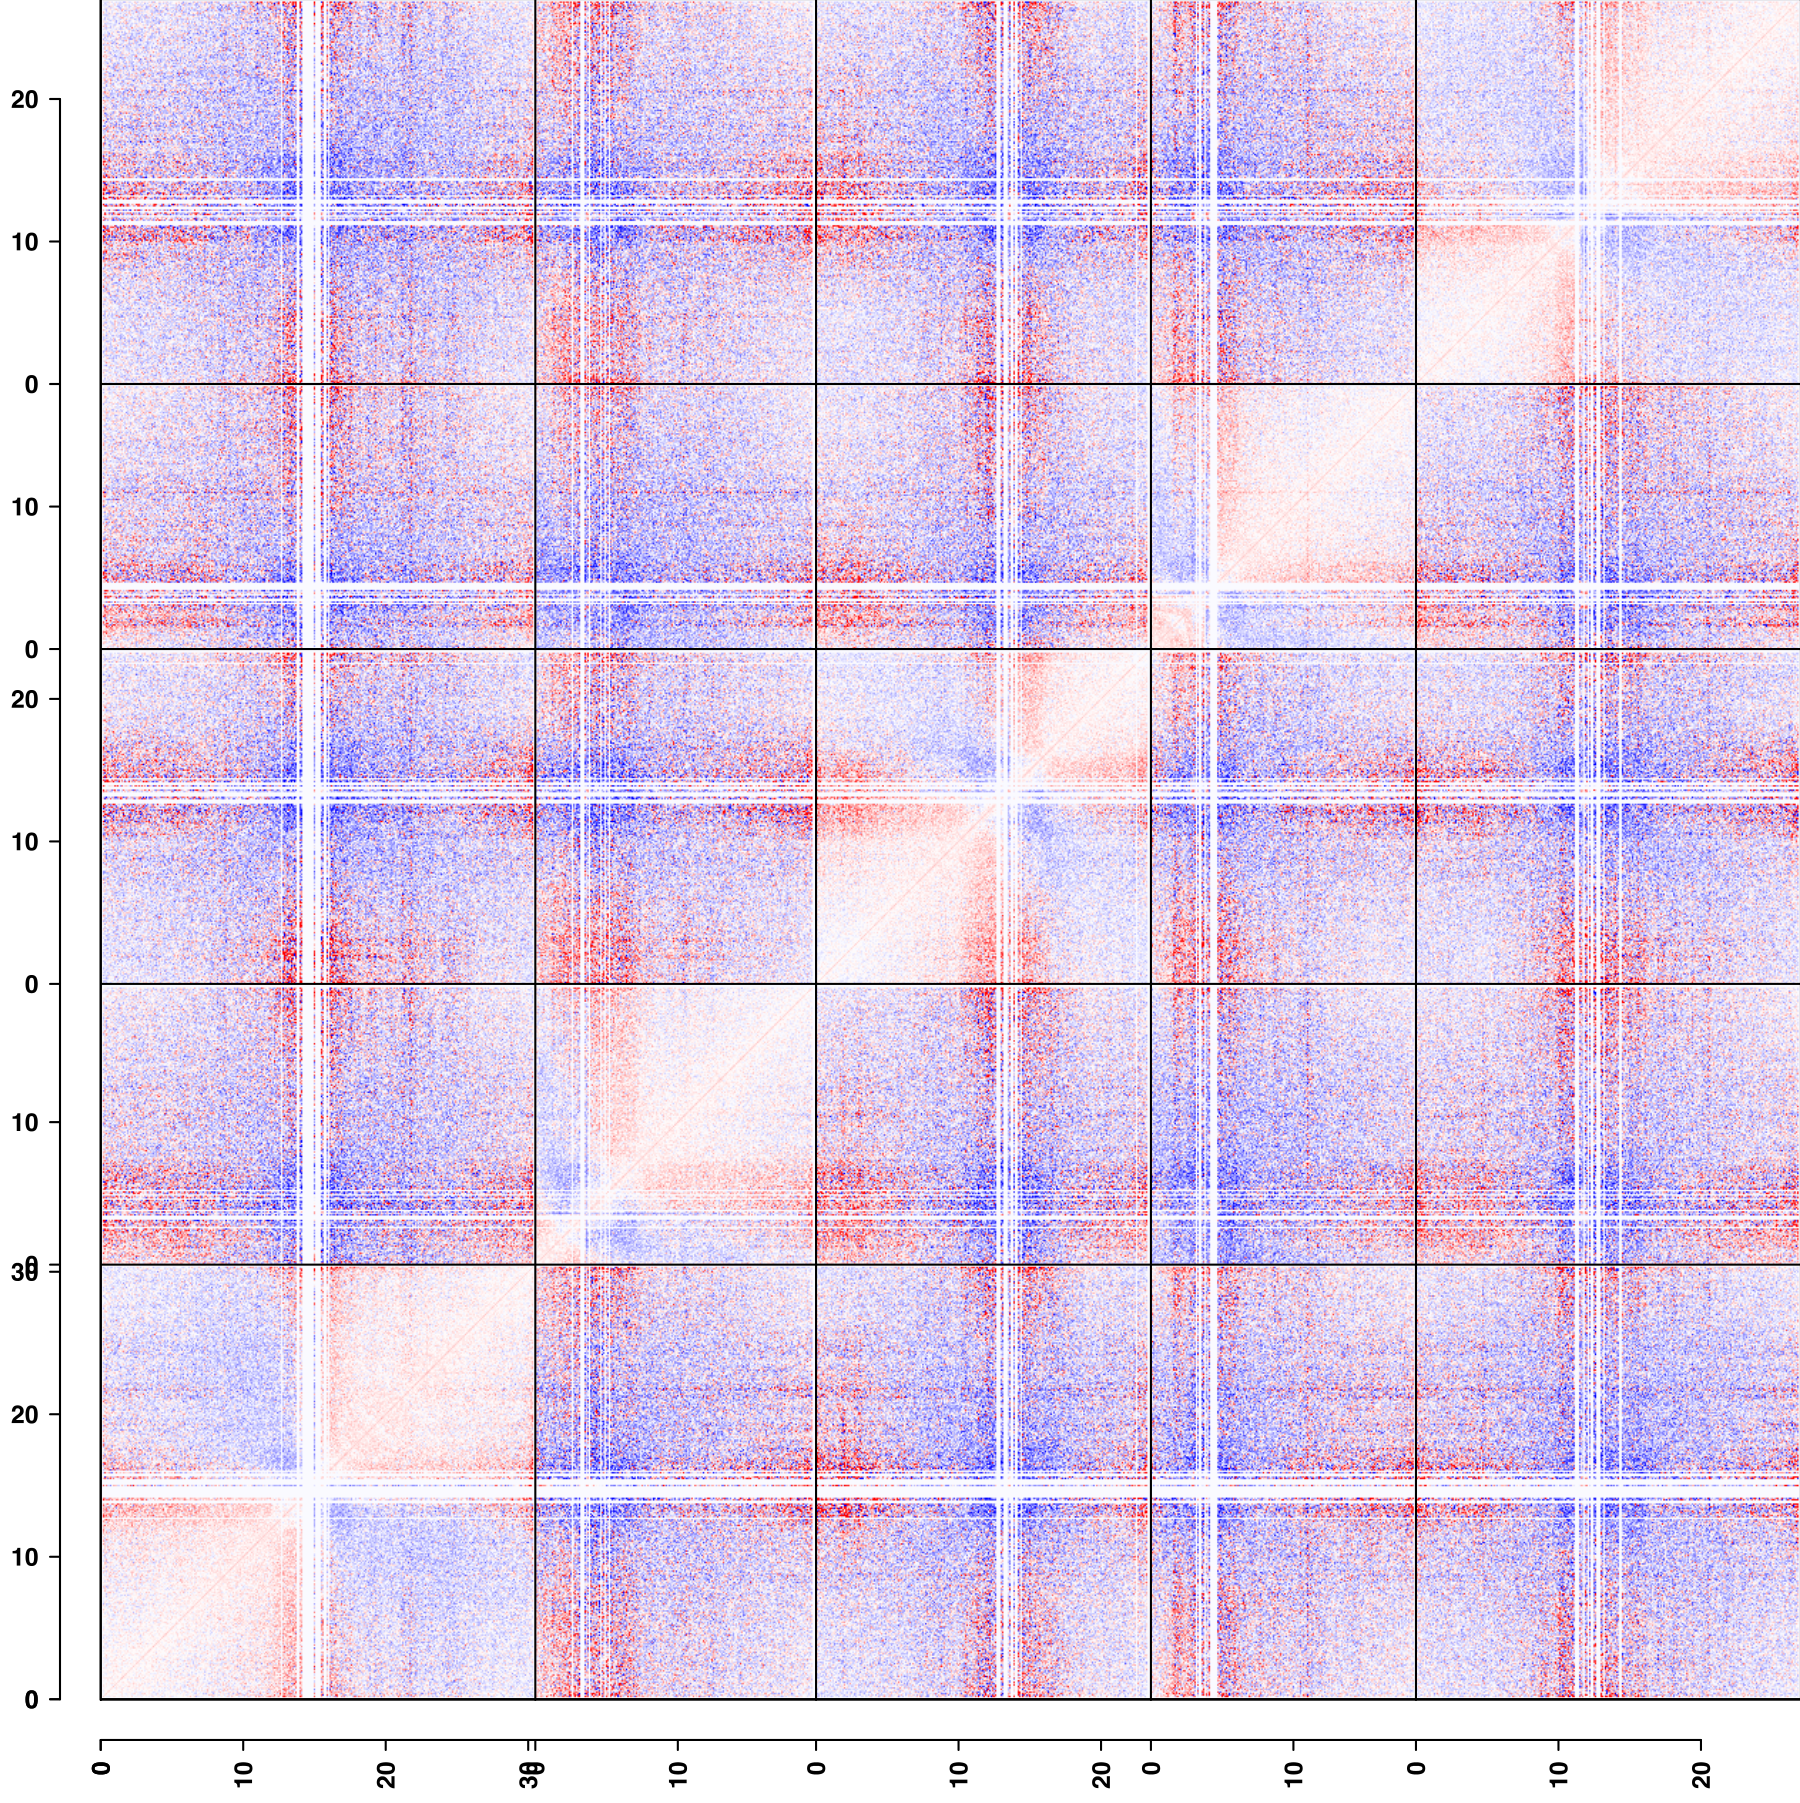
\includegraphics[width=5in]{relDiff_Col_crwn4.png}
\end{center}
\caption{Enrichment (blue) and depletion (red) of interaction frequencies in the wild-type compared to the \textit{crwn4} mutant sample of \textit{A. thaliana} \cite{2014_Grob} (100 kb bins).}
\label{relDiff}
\end{figure}
\clearpage
%%%%%%%%%%%%%%%%%%%%%%%%%%%%%%%%%%%%%%%%%%%%%%%%%%%%%%%%%%%%%%%%%%%%%%%%%%%%%%%%%%%%%%%%%%%%%%%%%%%%%%%%%%%%%%%%%%%%%%%%%%%%%%%%%%%%%%%%%%%%%%%%%%%%%%%%%%%%%%%%%%%%%%%%%%%%%%%%%%%%%%%%%%%%%%%%%%%%%%%%%%%%%%%%%%%%%%%%%%%%%%
\subsubsection{Comparison between Hi-C matrices - correlated differences}
To see if differences are clustered, the relative differences can be correlated to each other \cite{2014_Grob}. The correlation (i.e. a pixel at row $i$ and column $j$) is thereby calculated between two vectors of relative differences $C_{ij} = cor(R_{i},R_{j})$. A pair of Hi-C samples can be visualized using the function \texttt{f.plot.cor.difference()}. Multiple samples are compared to each other with \texttt{f.compare.samples.cor.difference()} (figure \ref{corDiff}).
\begin{verbatim}
f.plot.cor.difference(
    dataMatrixA = dataMatrixSampleA,
    dataMatrixB = dataMatrixSampleB,
    binSize = 1e6,
    rDir = "/path/to/where/the/figure/is/stored",
    outfile = "aNameForTheFigureWithoutExtension",
    filterZero = TRUE,
    filterThreshold = 0.95
)

f.compare.samples.cor.difference(
    dataMatrixList = dataMatrices,
    binSize = 1e6,
    rDir = "/path/to/where/the/figures/are/stored",
    outfilePrefix = "aPrefixForTheFileNames",
    filterZero = TRUE,
    filterThreshold = 0.95
)
\end{verbatim}
\begin{itemize}
 \item[-] \texttt{dataMatrixA, dataMatrixB} are two matrices created by \texttt{f.load.one.sample()}.
 \item[-] \texttt{dataMatrixList} is a list of n*n matrices created by \texttt{f.load.samples()}. 
 \item[-] \texttt{binSize} specifies the size of the genomic bins to be used (\texttt{binSize = 0} for restriction fragments).
 \item[-] \texttt{outfilePrefix ["corDiff\_"]} will be added in front of all file names.
 \item[-] \texttt{filterZero [TRUE]} tells whether or not to filter the x percent of bins with the highest number of 0 entries.
 \item[-] \texttt{filterThreshold [0.95]} specifies the fraction of bins which shall be kept if \texttt{filterZero = TRUE}.
\end{itemize}
\clearpage
\begin{figure}[!ht]
\begin{center}
\centering
\includegraphics[width=5in]{corDiff_Col_crwn4.png}
\end{center}
\caption{Correlation of differences between the wild-type and the \textit{crwn4} mutant samples of \textit{A. thaliana} \cite{2014_Grob} (100 kb bins).}
\label{corDiff}
\end{figure}
\clearpage
%%%%%%%%%%%%%%%%%%%%%%%%%%%%%%%%%%%%%%%%%%%%%%%%%%%%%%%%%%%%%%%%%%%%%%%%%%%%%%%%%%%%%%%%%%%%%%%%%%%%%%%%%%%%%%%%%%%%%%%%%%%%%%%%%%%%%%%%%%%%%%%%%%%%%%%%%%%%%%%%%%%%%%%%%%%%%%%%%%%%%%%%%%%%%%%%%%%%%%%%%%%%%%%%%%%%%%%%%%%%%%
\subsubsection{Comparison between Hi-C matrices - signed differences (SDM)}
An alternative way to assess the difference between two Hi-C samples are signed difference matrices (SDM) described in \cite{2014_Grob}. For each matrix entry (i.e. a pixel at row $i$ and column $j$), the signed difference indicates whether a given interaction is higher or lower in sample A than sample B: $B_{ij}=sign(A_{ij}-B_{ij})$. For a pair of Hi-C samples, these signed differences can be visualized and tested for being clustered (e.g. if sample A has higher interaction frequencies than sample B over a whole chromosome arm) using the function \texttt{f.plot.signed.difference()}. Multiple samples are compared to each other with \texttt{f.compare.samples.signed.difference()}  (figure \ref{sdmDiff}).
\begin{verbatim}
SDMresult <- f.plot.signed.difference(
    dataMatrixA = dataMatrixSampleA,
    dataMatrixB = dataMatrixSampleB,
    binSize = 1e6,
    rDir = "/path/to/where/the/figure/is/stored",
    outfile = "aNameForTheFigureWithoutExtension",
    filterZero = TRUE,
    filterThreshold = 0.95,
    pValueThreshold = 0.01
)

SDMresultList <- f.compare.samples.signed.difference(
    dataMatrixList = dataMatrices,
    binSize = 1e6,
    rDir = "/path/to/where/the/figures/are/stored",
    outfilePrefix = "aPrefixForTheFigureNames",
    filterZero = TRUE,
    filterThreshold = 0.95,
    pValueThreshold = 0.01
)
\end{verbatim}
\begin{itemize}
 \item[-] \texttt{SDMresult} is an object holding the overall P-value (\texttt{SDMresult\$overallPvalue}) and the significant bin IDs (\texttt{SDMresult\$significantRows}). 
 \item[-] \texttt{SDMresultList} is a list of objects created by \texttt{f.plot.signed.difference()}.
 \item[-] \texttt{dataMatrixA, dataMatrixB} are two matrices created by \texttt{f.load.one.sample()}.
 \item[-] \texttt{dataMatrixList} is a list of n*n matrices created by \texttt{f.load.samples()}. 
 \item[-] \texttt{binSize} specifies the size of the genomic bins to be used (\texttt{binSize = 0} for restriction fragments).
 \item[-] \texttt{outfilePrefix ["relDiff\_"]} will be added in front of all file names.
 \item[-] \texttt{filterZero [TRUE]} tells whether or not to filter the x percent of bins with the highest number of 0 entries.
 \item[-] \texttt{filterThreshold [0.95]} specifies the fraction of bins which shall be kept if \texttt{filterZero = TRUE}.
 \item[-] \texttt{pValueThreshold [0.01]} specifies the significance-threshold for the individual bins.
\end{itemize}
\clearpage
\begin{figure}[!ht]
\begin{center}
\centering
\includegraphics[width=5in]{sdmDiff_Col_crwn4.png}
\end{center}
\caption{Visualization of the difference between the wild-type and \textit{crwn4} mutant samples of \textit{A. thaliana} \cite{2014_Grob} using the signed difference matrix (100 kb bins).}
\label{sdmDiff}
\end{figure}
\clearpage
%%%%%%%%%%%%%%%%%%%%%%%%%%%%%%%%%%%%%%%%%%%%%%%%%%%%%%%%%%%%%%%%%%%%%%%%%%%%%%%%%%%%%%%%%%%%%%%%%%%%%%%%%%%%%%%%%%%%%%%%%%%%%%%%%%%%%%%%%%%%%%%%%%%%%%%%%%%%%%%%%%%%%%%%%%%%%%%%%%%%%%%%%%%%%%%%%%%%%%%%%%%%%%%%%%%%%%%%%%%%%%
\subsubsection{Distance-dependent decay of interaction frequencies}
The distance-dependent decay of interaction frequencies (IDEs, as described in \cite{2009_LiebermanAiden}) within a Hi-C sample can be calculated and visualized using the function \texttt{f.distance.decay()} (figue \ref{distanceDecay}).
\begin{verbatim}
f.distance.decay(
    dataMatrix = dataMatrixSampleX,
    binSize = 1e6,
    rDir = "/path/to/where/the/figure/is/stored",
    outfile = "aNameForTheFigureWithoutExtension",
    distance = 10e6,
    regionTable = data.frame(),
    filterZero = TRUE,
    filterThreshold = 0.95
)
\end{verbatim}
\begin{itemize}
 \item[-] \texttt{dataMatrix} is a matrix created by \texttt{f.load.one.sample()}.
 \item[-] \texttt{binSize} specifies the size of the genomic bins to be used (must be greater than zero, i.e. the function only takes bins with a fixed size).
 \item[-] \texttt{distance} specifies the distance up to which the interaction frequency decay shall be considered. Must be smaller than the smallest region (e.g. smaller than the smalles chromosome if \texttt{regionTable = data.frame()})
 \item[-] \texttt{regionTable [data.frame()]} defines specific regions in the genome which shall be assessed. Per default, each chromosome is first tested separately and a common IDE is calculated as the average between all individual IDEs. The table must have three columns (\texttt{chrom, start, end}). User defined names can be given using an optional fourth column (\texttt{name}). An example is given in the \textit{A. thaliana} tutorial.
 \item[-] \texttt{filterZero [TRUE]} tells whether or not to filter the x percent of bins with the highest number of 0 entries.
 \item[-] \texttt{filterThreshold [0.95]} specifies the fraction of bins which shall be kept if \texttt{filterZero = TRUE}.
\end{itemize}
\clearpage
\begin{figure}[!ht]
\begin{center}
\centering
\includegraphics[width=4in]{mergedDD.png}
\end{center}
\caption{Distance-dependent decay of interaction frequencies along entire chromosomes (10 mb, top panel), euchromatic parts of chromosome arms (5 mb, middle panel), and heterochromatic pericentromeres (1 mb, lower panel) in a pooled wild-type sample of \textit{A. thaliana} \cite{2012_Moissiard,2014_Grob} (100 kb bins).}
\label{distanceDecay}
\end{figure}
\clearpage
%%%%%%%%%%%%%%%%%%%%%%%%%%%%%%%%%%%%%%%%%%%%%%%%%%%%%%%%%%%%%%%%%%%%%%%%%%%%%%%%%%%%%%%%%%%%%%%%%%%%%%%%%%%%%%%%%%%%%%%%%%%%%%%%%%%%%%%%%%%%%%%%%%%%%%%%%%%%%%%%%%%%%%%%%%%%%%%%%%%%%%%%%%%%%%%%%%%%%%%%%%%%%%%%%%%%%%%%%%%%%%
\subsubsection{Reading the annotation}\label{annotationLoading}
Fragment annotations (additional tracks with genomic and epigenetic information) processed with \textit{HiCdatPre} can be read into R using the function \texttt{f.read.annotation()}. Annotations for genomic bins with fixed size can also be obtained from annotated restriction fragments with \texttt{f.read.annotation.via.fragment.annotation()}.
\begin{verbatim}
annotation <- f.read.annotation(
    annotationFile = "/path/to/file/created/with/HiCdatPre", 
    binSize = 1e6, 
    useLog = TRUE
)

annotation <- f.read.annotation.via.fragment.annotation(
    annotationFile = "/path/to/file/created/with/HiCdatPre", 
    binSize = 1e6, 
    useLog = TRUE
)
\end{verbatim}
\begin{itemize}
 \item[-] \texttt{annotation} is a table holding genomic and epigenetic information (see \textit{HiCdatPre}, section \ref{HiCdat}).
 \item[-] \texttt{binSize} specifies the size of the genomic bins to be used (\texttt{binSize = 0} for restriction fragments in \texttt{f.read.annotation()}).
 \item[-] \texttt{useLog [TRUE]} specifies if count-like features (columns starting with \texttt{ann\_, sum\_}) shall be transformed using \texttt{log2(data + 1)}.
\end{itemize}
\clearpage
%%%%%%%%%%%%%%%%%%%%%%%%%%%%%%%%%%%%%%%%%%%%%%%%%%%%%%%%%%%%%%%%%%%%%%%%%%%%%%%%%%%%%%%%%%%%%%%%%%%%%%%%%%%%%%%%%%%%%%%%%%%%%%%%%%%%%%%%%%%%%%%%%%%%%%%%%%%%%%%%%%%%%%%%%%%%%%%%%%%%%%%%%%%%%%%%%%%%%%%%%%%%%%%%%%%%%%%%%%%%%%
\subsubsection{Analysis of the first principle component (PCA)}
Analysis of the first principle component can be used as a tool to identify discrete structural domains \cite{2009_LiebermanAiden}. The first principle component can be obtained and related to the genomic and epigenetic features (annotation) using the function \texttt{f.principle.component.analysis.and.features()} (figure \ref{PCA}). Note that the function tries to orient the first principle component as such that positive Eigenvalues correspond to more loose (and negative Eigenvalues to a more compact) chromatin configuration.
\begin{verbatim}
f.principle.component.analysis.and.features(
    dataMatrix = dataMatrixSampleX,
    binSize = 1e6,
    rDir = "/path/to/where/the/results/are/stored",
    outfilePrefix = "aPrefixForTheFileNames",
    annotation = annotationTable, # or data.frame() if only PCA is requested
    regionTable = data.frame(),
    simplifiedNames = list(),
    filterZero = TRUE,
    filterThreshold = 0.95,
    pValueThreshold = 0.05,
    userLimits = c(-1, 1)
)
\end{verbatim}
\begin{itemize}
 \item[-] \texttt{dataMatrix} is a matrix created by \texttt{f.load.one.sample()}.
 \item[-] \texttt{binSize} specifies the size of the genomic bins to be used (must be greater than zero, i.e. the function only takes bins with a fixed size).
 \item[-] \texttt{annotation [data.frame()]} is a table holding genomic and epigenetic information, loaded with \texttt{f.read.annotation()}. If no annotation is supplied, the function only performs the PCA.
 \item[-] \texttt{regionTable [data.frame()]} defines specific regions in the genome which shall be analyzed individually. Per default, each chromosome is tested separately. The table must have three columns (\texttt{chrom, start, end}). User defined names can be given using an optional fourth column (\texttt{name}). An example is given in the \textit{A. thaliana} tutorial.
 \item[-] \texttt{simplifiedNames [list()]} is a list with the column names of the annotation as keys to simplified names as values (e.g. ``ann\_transposable\_element\_gene'' can be replaced by ``TE-gene'').
 \item[-] \texttt{filterZero [TRUE]} tells whether or not to filter the x percent of bins with the highest number of 0 entries.
 \item[-] \texttt{filterThreshold [0.95]} specifies the fraction of bins which shall be kept if \texttt{filterZero = TRUE}.
 \item[-] \texttt{pValueThreshold [0.05]} specifies the significance-threshold for the correlation and enrichment tests (only significant values are drawn in the heatmaps).
 \item[-] \texttt{userLimits [c(-1, 1)]} specifies the lower and upper limit for the correlation values drawn in the heatmap.
\end{itemize}
\clearpage
\begin{figure}[!ht]
\begin{center}
\centering
\includegraphics[width=3.5in]{PCA.png}
\end{center}
\caption{Left panels: Visualization of distance-normalized and correlated Hi-C interaction frequencies and the resulting first principle component. Middle: significant correlation (blue: positive, red: negative) of the first principle component with various genomic and epigenetic features. Right: significant enrichment (blue) and depletion (red) of genomic and epigenetic features in regions with positive Eigenvalues compared to regions with negative Eigenvalues. Data shown for the right arms of chromosomes 1, 4, and 5 from a pooled wild-type sample of \textit{A. thaliana} \cite{2012_Moissiard,2014_Grob} (100 kb bins).}
\label{PCA}
\end{figure}
\clearpage
%%%%%%%%%%%%%%%%%%%%%%%%%%%%%%%%%%%%%%%%%%%%%%%%%%%%%%%%%%%%%%%%%%%%%%%%%%%%%%%%%%%%%%%%%%%%%%%%%%%%%%%%%%%%%%%%%%%%%%%%%%%%%%%%%%%%%%%%%%%%%%%%%%%%%%%%%%%%%%%%%%%%%%%%%%%%%%%%%%%%%%%%%%%%%%%%%%%%%%%%%%%%%%%%%%%%%%%%%%%%%%
\subsubsection{Test a specific set of bins for higher interaction among each other}
A given set of genomic regions can be tested for preferential interaction among each other compared to sets of randomly sampled regions using the function \texttt{f.test.interaction.frequencies()}.
\begin{verbatim}
f.test.interaction.frequencies(
    dataMatrix = dataMatrixSampleX,
    binSize = 1e6,
    repetitions = 1e4,
    testRegionsTable = tableWithRegionsOfInterest,
    regionDefinitionTable = data.frame()
)
\end{verbatim}
\begin{itemize}
 \item[-] \texttt{interactionResult} is a vector holding the sum of interactions between the regions of interest, the mean and standard deviation of the sampled interaction sums, and the corresponding P-value.
 \item[-] \texttt{dataMatrix} is a matrix created by \texttt{f.load.one.sample()}.
 \item[-] \texttt{binSize} specifies the size of the genomic bins to be used (must be greater than zero, i.e. the function only takes bins with a fixed size).
 \item[-] \texttt{repetitions} specifies the number of random sets to be sampled.
 \item[-] \texttt{testRegionsTable} is a table with genomic regions of interest. Columns must be \texttt{chrom, start, end}. Rownames can be freely chosen. An example is given in the \textit{A. thaliana} tutorial.
 \item[-] \texttt{regionDefinitionTable} defines specific regions in the genome from which the random sets are sampled. If a table is supplied, the regions of interest are assigned to the defined regions (unassigned will be removed) and sampling happens within the defined region (see \cite{2014_Grob} for details). If no regions are defined, the regions of interest are assigned to the whole chromosomes. Mapping of regions is done on the whole length (a test region must be entirely within a defined region to be assigned to it - unassigned test regions are removed). The table must have three columns (\texttt{chrom, start, end}). User defined names can be given using an optional fourth column (\texttt{name}). An example is given in the \textit{A. thaliana} tutorial.
\end{itemize}
\clearpage
%%%%%%%%%%%%%%%%%%%%%%%%%%%%%%%%%%%%%%%%%%%%%%%%%%%%%%%%%%%%%%%%%%%%%%%%%%%%%%%%%%%%%%%%%%%%%%%%%%%%%%%%%%%%%%%%%%%%%%%%%%%%%%%%%%%%%%%%%%%%%%%%%%%%%%%%%%%%%%%%%%%%%%%%%%%%%%%%%%%%%%%%%%%%%%%%%%%%%%%%%%%%%%%%%%%%%%%%%%%%%%
\subsubsection{Test a specific set of bins for enrichment/depletion of certain annotation features}
A given set of genomic regions can further be tested for enrichment or depletion of certain genomic or epigenetic features using the function \texttt{f.test.regions.for.feature.enrichment.fragment.based()}.
\begin{verbatim}
enrichmentResult <- f.test.regions.for.feature.enrichment.fragment.based(
    annotation = annotationTableOnRestrictionFragments,
    rDir = "/path/to/where/the/results/are/stored",
    outfilePrefix = "aPrefixForTheFileNames",
    repetitions = 1e4,
    testRegionsTable = tableWithRegionsOfInterest,
    regionDefinitionTable = data.frame(),
    simplifiedNames = list(),
    pValueThreshold = 0.05,
    countDataWasLogged = TRUE
)
\end{verbatim}
\begin{itemize}
 \item[-] \texttt{enrichmentResult} is a list holding the observed values (\texttt{enrichmentResult\$observed}), the enrichment (\texttt{enrichmentResult\$enrichment}) compared to the random sets, and the corresponding P-values (\texttt{enrichmentResult\$pValues}).
 \item[-] \texttt{annotation} is a table holding genomic and epigenetic information, loaded with \texttt{f.read.annotation(..., binSize = 0)}. It is important that the annotation is based on restriction fragments and not genomic bins with fixed size (for the latter case, it is possible, but not recommended, to use \texttt{f.test.regions.for.feature.enrichment.bin.based})
 \item[-] \texttt{repetitions} specifies the number of random sets to be sampled.
 \item[-] \texttt{testRegionsTable} is a table with genomic regions of interest. Columns must be \texttt{chrom, start, end}. Rownames can be freely chosen. An example is given in the \textit{A. thaliana} tutorial.
 \item[-] \texttt{regionDefinitionTable} defines specific regions in the genome from which the random sets are sampled. If a table is supplied, the regions of interest are assigned to the defined regions (unassigned will be removed) and sampling happens within the defined region (see \cite{2014_Grob} for details). If no regions are defined, the regions of interest are assigned to the whole chromosomes. Mapping of regions is done on the whole length (a test region must be entirely within a defined region to be assigned to it - unassigned test regions are removed). The table must have three columns (\texttt{chrom, start, end}). User defined names can be given using an optional fourth column (\texttt{name}). An example is given in the \textit{A. thaliana} tutorial.
 \item[-] \texttt{simplifiedNames [list()]} is a list with the column names of the annotation as keys to simplified names as values (e.g. ``ann\_transposable\_element\_gene'' can be replaced by ``TE-gene'').
 \item[-] \texttt{pValueThreshold [0.05]} specifies the significance-threshold for the enrichment tests (only significant values are drawn in the heatmaps).
 \item[-] \texttt{countDataWasLogged [TRUE]} tells if \texttt{useLog = TRUE} while loading the annotation with \texttt{f.load.annotation()}.
\end{itemize}
\clearpage
%%%%%%%%%%%%%%%%%%%%%%%%%%%%%%%%%%%%%%%%%%%%%%%%%%%%%%%%%%%%%%%%%%%%%%%%%%%%%%%%%%%%%%%%%%%%%%%%%%%%%%%%%%%%%%%%%%%%%%%%%%%%%%%%%%%%%%%%%%%%%%%%%%%%%%%%%%%%%%%%%%%%%%%%%%%%%%%%%%%%%%%%%%%%%%%%%%%%%%%%%%%%%%%%%%%%%%%%%%%%%%
\subsubsection{Identify domains within chromosomes with HiCseg}
Domains within chromosomes (e.g., TADs) can be identified using the HiCseg package described in \cite{2014_LevyLeduc}. To use it, you need to first install the HiCseg package (\texttt{install.packages("HiCseg")}). The function \texttt{f.identify.domains.with.HiCseg()} is a wrapper for the HiCseg package.
\begin{verbatim}
domainResults <- f.identify.domains.with.HiCseg(
    dataMatrix = dataMatrixSampleX,
    binSize = 1e5,
    rDir = "/path/to/where/the/results/are/stored",
    outfilePrefix = "aPrefixForTheFileNames",
    minAverageDomainSize = 1e6,
    distributionType = "G",
    modelType = "D",
    useLog = FALSE,
    regionDefinitionTable = data.frame()
)
\end{verbatim}
\begin{itemize}
 \item[-] \texttt{dataMatrix} is a matrix created by \texttt{f.load.one.sample()}.
 \item[-] \texttt{binSize} specifies the size of the genomic bins to be used (\texttt{binSize = 0} for restriction fragments).
 \item[-] \texttt{minAverageDomainSize} is the minimal average domain size in base pairs. This argument is used to calculate the maximal number of domains within a chromosome given its size.
 \item[-] \texttt{distributionType} describes the distribution of the data: ``B'' is for Negative Binomial distribution, ``P'' is for the Poisson distribution, and ``G'' is for the Gaussian distribution. In general, take Gaussian for normalized data and Poisson/Negative Binomial for raw data..
 \item[-] \texttt{modelType} "D" for block-diagonal and "Dplus" for the extended block-diagonal model (see \cite{2014_LevyLeduc} for details).
 \item[-] \texttt{useLog [TRUE]} tells if the data shall be transformed using \texttt{log2(data + 1)}.
 \item[-] \texttt{regionDefinitionTable} defines specific regions in the genome where domains shall be searched. If no regions are defined, domains are searched on the entire chromosomes. The table must have three columns (\texttt{chrom, start, end}). User defined names can be given using an optional fourth column (\texttt{name}).
\end{itemize}
\clearpage
% \begin{figure}[!ht]
% \begin{center}
% \centering
% \includegraphics[width=5in]{KEE.png}
% \end{center}
% \caption{}
% \label{KEEenrichment}
% \end{figure}
% \clearpage
%%%%%%%%%%%%%%%%%%%%%%%%%%%%%%%%%%%%%%%%%%%%%%%%%%%%%%%%%%%%%%%%%%%%%%%%%%%%%%%%%%%%%%%%%%%%%%%%%%%%%%%%%%%%%%%%%%%%%%%%%%%%%%%%%%%%%%%%%%%%%%%%%%%%%%%%%%%%%%%%%%%%%%%%%%%%%%%%%%%%%%%%%%%%%%%%%%%%%%%%%%%%%%%%%%%%%%%%%%%%%%
\section{Building from source}\label{buildInstructions}
If the binary is not working or you would like to implement a new feature, you can build it from the source code. 
\subsection{Linux}
Compiling the program using QtCreator is quite easy.
\begin{itemize}
\item download and unpack the archive \texttt{source.zip}
\item install QtCreator (on the Ubuntu repository: \texttt{qtcreator}) - make sure to use Qt 4.x.x libraries
\item install zlib (on the Ubuntu repository: \texttt{zlib1g}, \texttt{zlib1g-dev}, \texttt{zlib1g-dev})
\item start QtCreator and open the \texttt{../source/HiCdatPre.pro} file 
\item copy the seqan folder into one of your general include paths (e.g. \texttt{sudo cp -r seqan /usr/local/include}) or add a line \texttt{INCLUDEPATH += <path containing seqan folder>} into the *.pro file
\item finally, in the QtCreater menu select \texttt{Build > Build Project ``my\_project''}
\end{itemize}
\subsection{Windows}
Compiling on Windows requires access to VisualStudio. The following steps worked well with VisualStudio 2010 Ultimate.
\begin{itemize}
\item download and unpack the archive \texttt{source.zip}
\item install the Qt Add-In for VisualStudio - make sure to use Qt 4.x.x libraries
\item open the \texttt{../source/HiCdatPre.pro} file  (\texttt{Qt > Open Qt Project File (.pro)...})
\item download the latest zlib from zlib.net (e.g. \texttt{zlib-1.2.8.tar.gz}) and unpack the archive
\item open the project properties (right-click on the project in the solution explorer) and do the following steps:
\begin{itemize}
\item under \texttt{Configuration Properties > VC++ Directories}, in the field \texttt{Include Directories}, add the zlib folder
\item under \texttt{Configuration Properties > VC++ Directories}, in the field \texttt{Include Directories}, add the folder containing the seqan folder
\item under \texttt{Configuration Properties > General}, change the variable \texttt{Character Set} to \texttt{Use Multi-Byte Character Set}
\item under \texttt{Configuration Properties > C/C++ > Preprocessor} in the field \texttt{Preprocessor Definitions}, remove the \texttt{UNICODE} key-words and add the key-word \texttt{\_CRT\_SECURE\_NO\_WARNINGS}
\item under \texttt{Configuration Properties > C/C++ > Command Line}, add the options \texttt{-W2 -wd4996} in the field with the \texttt{Additional Options}
\end{itemize}
\item close the project properties and compile it with \texttt{Build > Build Solution}
\end{itemize}
\subsection{Mac}
Currently, there are no build instructions available for the MacOS.
% due to Qt 5 instead of 4: #include <QtWidgets> wherever one has #include <QtGui>; in the pro file QT += ... widgets; in main.cpp #include <QtGui/QApplication> becomes to #include <QtWidgets/QApplication> 
% also due to Qt: QChar ...toAscii() replaced by toLatin1()
% in the .pro file INCLUDEPATH+= ../zlib-1.2.8 \ ../ and LIBS += -lZ
% in main.cpp before QApplication a(...), add the lines:
%     QString path = QString(argv[0]);
%     QString end = path.split("/").last();
%     path.remove(path.length() - end.length(), end.length());
%     QDir dir(path);
%     dir.cdUp();
%     dir.cd("PlugIns");
%     QApplication::setLibraryPaths(QStringList(dir.absolutePath()));
% then: /Users/stefan/Applications/Qt/5.3/clang_64/bin/macdeployqt xy.app -always-overwrite -dmg
% With QT 5.4 instead of 5.3: macdeployqt <TARGET>.app -executable=<TARGET>.app/Contents/MacOS/<TARGET>  -always-overwrite -dmg
%\bibliographystyle{elsart-harv}
\bibliography{userGuideReferences}
\bibliographystyle{elsart-num}
\end{document}
